
\chapter{EXISTING WORKS}
\label{ch:ExistingWorks}

In Section \ref{sec:Objectives} we listed seven design requirements that ideally must be met by a naming system in order to be applicable to Tor hidden services. We now examine several workarounds and existing naming systems against these objectives.

\section{Address Manipulation}

Although they are not separate naming systems in their own right, several systems have been proposed to directly improve the readability of hidden service addresses. These include vanity key generators and different encoding schemes.

Shallot is a vanity key generator which uses OpenSSL to generate by brute-force many RSA keys in attempt to find one that has a desirable hash.\cite{KatmagicShallot} For example, a hidden service operator may wish to start his service's address with a meaningful noun so that others may more easily recognize it. Shallot has been used successfully for both common and high-profile hidden services, such as blockchainbdgpzk.onion, an official mirror of Blockchain.info; facebookcorewwwi.onion, Facebook's hidden services; and  freepress3xxs3hk.onion, the Freedom of the Press's SecureDrop instance. However, Shallot is only partially successful at enhancing readability because the size of the domain key-space is too large to be fully brute-forced in any reasonable length of time.\cite{KatmagicShallot} This situation is expected to get worse over time as Tor plans to increase the length of hidden service addresses.\cite{Proposal224} If the address key-space was reduced to allow a full brute-force, the system would fail to be guaranteed collision-free.

Nicolussi suggested changing the address encoding from base58 to a delimited series of words, using a dictionary known in advance by all parties.\cite{nicolussi2011human} We consider this approach very similar to vanity key generation. Like Shallot, Nicolussi's encoding partially improves the recognition and readability of an address but does nothing to alleviate the logistic problems of manually entering in the address into the Tor Browser. The key-space is not changed and is again too large for hidden service operators to select many meaningful words.

These proposals are cosmetic and do not significantly change Tor's hidden service infrastructure and its intersection with our design requirements; they still support anonymous registrations, privacy-enhanced lookups, publicly verifiable registrations, collision-free addresses, and are distributed by nature. However, they only meet one side of Zooko's Triangle and thus fail our usability requirements; although these are partial solutions, they do not achieve a full correlation between an address and the service's purpose.

\section{Centralized or Zone-Based DNS}

\subsection{Internet DNS}

The Internet's Domain Name System was designed in 1983 to map Internet domain names to IP addresses. A domain name consists of a series of labels, delimited by dots. Each label subdivides the system into hierarchical zones, where the root zone that contains TLDs (top-level domains such as .com, .org, or .gov) is managed by IANA and NTIA. Each label can be up to 63 characters in length with the entire domain name up to 253 characters in length. The Internet DNS is a critical component to the usability of the Internet as it abstracts away IP addresses, allowing servers to be referenced by an easily-memorized human-meaningful name.

Despite its widespread use and extreme popularity, the Internet DNS suffers from several significant shortcomings and security issues that make it inappropriate for use by Tor hidden services. With the exception of extensions such as DNSSEC, the Internet DNS by default does not use any cryptographic primitives. However, as DNSSEC is primarily designed to prevent forgeries and DNS cache poisoning from intermediary DNS resolvers, it preserves the hierarchical structure and does not provide any degree of query privacy.\cite{wachs2014censorship} Additional extensions and protocols such as DNSCurve\cite{bernstein2009dnscurve} have been proposed, but DNSSEC and DNSCurve are optional and have not yet seen widespread full deployment across the Internet. Traditional DNS lookups may be intercepted and modified by MITM attacks, user privacy may be compromised by wiretapping DNS lookups, and the system is by default vulnerable to DNS cache poisoning.

The lack of default security in Internet DNS and the financial expenses involved with registering a new TLD casts significant doubt on the feasibility of using for Tor hidden services. Furthermore the system meets only a few of our design requirements: although the system is easy to use, the system is hierarchical but not truly distributed, domain registrars typically require the owner to reveal significant amounts of identifiable information, registrations are not confirmable except through expensive SSL certificates issues by a central authority, and lookups occur by default without any privacy enhancements. These issues make the Internet DNS ill-suited for Tor hidden services.

\subsection{GNU Name System}

The GNU Name System\cite{wachs2014censorship} (GNS) is a decentralized privacy-enhanced replacement for the Internet DNS. GNU describes a hierarchical zones of with each user managing their own zone and distributing zone access peer-to-peer within social circles without any central authority. Every GNS use (let Alice be one such user) chooses a nickname for themselves which they announce to the network via a distributed hashtable. A peer Bob selects a name for Alice, which is typically Alice's nickname unless there is a collision. Then Bob adds Alice's zone into his zone such that he delegates all requests for her nickname to Alice. In this way, Bob acts as a resolver to Alice and Bob's name for Alice (or her nickname for herself) is guaranteed unique within Bob's zone. Bob's peers can likewise add Bob and Alice's zone to their zone and delegate requests for them. Assuming each user has selected a unique name for themselves, (which they are incentivized to do) there will be no collusions within each zone. GNS uses the .gnu pseudo-TLD.

While GNS' design guarantees the uniqueness of names within each zone and users are capable of selecting meaningful nicknames for themselves, GNU does not guarantee that names are \emph{globally} unique. The selection of a trustworthy zone to use would be a significant challenge for using GNS for Tor hidden services. The user maintaining that zone is a central point of failure and could severerly disrupt the system if they acted maliciously. However, GNS does support anonymous registrations, privacy-enhanced queries, authenticated domain names, simplicity, and backwards compatibility. For these reasons, we consider GNS a very impressive system and recommend GNS as a possible fallback from OnioNS.

\section{Distributed Systems}

Several systems have been developed that aim to serve names in a decentralized environment. Cachin and Samar\cite{cachin2004secure} extended the Internet DNS and decreased the attack potential for authoritative name servers via threshold cryptography, but the lack of privacy in the Internet DNS and the logistical difficulty in globally implementing their work prevents us from using their system for hidden services. Awerbuch and Scheideler,\cite{awerbuch2004group} constructed a distributed peer-to-peer naming system, but like GNS, made no guarantee that domain names would be globally unique. More recently, Zooko's Triangle was proven false by practical demonstration by the development of Namecoin, a cryptocurrency discussed below.

\subsection{Namecoin}
\label{sec:Namecoin}

Namecoin is a decentralized information registration and transfer system, developed pseudo-anonymously in early 2011. It was the first fork of Bitcoin\cite{nakamoto2008bitcoin} and inherits most of Bitcoin's design and capabilities. Namecoin holds digitally-signed information transactions in a data structure known as a block; each block links to a previous block, forming a public ledger known as a blockchain. Each participant in the Namecoin network holds a copy of the blockchain and listen for and broadcast new blocks peer-to-peer. New Namecoins are generated at a fixed rate in a process known as mining, which is the computationally-expensive generation (due to proof-of-work) of a new block. Namecoins are then transferred peer-to-peer, and the registration of a domain name has some cost as it consumes a quantity of Namecoins. Domain names use the .bit pseudo-TLD and expire approximately every 250 days and so must be renewed periodically to preserve exclusive ownership. In 2014, Namecoin was recognized by ICANN as the most well-known example of a PKI and DNS system with an emphasis of distributed control and privacy.\cite{NamecoinReportICANN}

\begin{figure}[htbp]
	\centering
	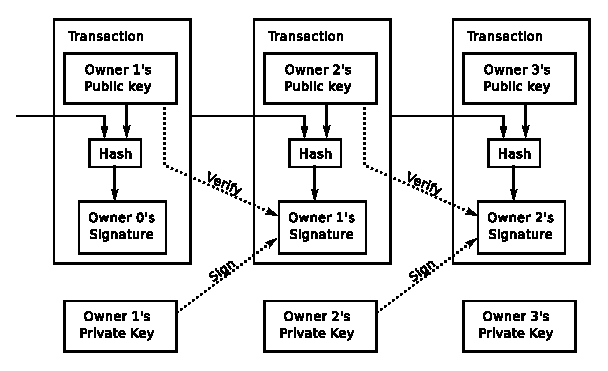
\includegraphics[width=0.7\textwidth]{images/Namecoin/bitcoin_transaction.eps}
	\caption{Three Namecoin transactions. Each owner broadcasts a digitally signed transaction that moves Namecoins from one ECDSA key to another. Every participant in the Namecoin network can validate the transaction by examine the blockchain and tracing ownership back to the point of origin.}
	\label{fig:NamecoinTransaction}
\end{figure}

As previously stated, Namecoin is noteworthy for being the first naming system to demonstratively achieve all three properties of Zooko's Triangle. It supports privacy-enhanced lookups as anyone can obtain a copy of the blockchain and perform queries against it, names are guaranteed to be unique as each participant (and thus the network as a whole) will reject new blocks that contain names already contained in their blockchain, and it is distributed by nature. While Namecoin is often advertised as capable of assigning names to Tor hidden services, it has several practical issues that make it generally infeasible to be used for that purpose and it fails several of our design requirements. First, to authenticate registrations, clients must be able to prove the relationship between a Namecoin owner's secp256k1 ECDSA key and the target hidden service's RSA key: constructing this relationship is non-trivial. Second, Namecoin generally requires users to download the blockchain before use which introduces logistical issues; as of April 2015 Namecoin's blockchain is 2.45 GB.\cite{BitInfoCharts} Third, although ownership and transfer of Namecoins leaks no more than an ECDSA key, obtaining the Namecoins in the first place (and thus being able to claim a domain name) anonymously is non-trivial due to the logging in the blockchain. Finally, unlike the aforementioned naming systems, Namecoin is not based on published works and literature on it is sparse. Although we also reject Namecoin as a possible naming system for Tor hidden services, OnioNS' design shares some design principles with Namecoin.
